
\documentclass[11pt,final]{article}
\usepackage{graphicx}

\title{Note : Stoichiometric Modelling of Cell Metabollism}
\author{Pottiez Thomas}
\date{\today}



\begin{document}
\maketitle
\section{Résumé}

Il y a plusieurs méthode pour représenter le métabolisme d'une cellule qui partage deux caractéristique : utilisation du réseau métabolique et assumer un pseudo état stationnaire.\\ Il existe plusieurs plusieurs méthode mathématique assumant différente chose. Dans ce papier le terme
"Modélisation Stochoimétrique"regroupe l'ensemble de ces méthode sous un framework mathématique commun.\\
Ce framework essaie de ce passer des informations relative aux réactions stochiométrique en utilisant une perspective basée sur la contrainte. Cela permet de ce passer du dévellopement d'un modèle cinétique car les prises de mesures relatives au paramètre de ce modèle sont complexe.\\

\section{Introduction}
Le comportement d'une cellule ne peut pas seulement être expliquer par les constituants de la cellule. Pour prédire son comportement, il faut prendre en compte les intéractions entre les éléments eux-même.\\
\[
   \frac{d M_i}{dt} = S \cdot v - \mu \cdot x => S \cdot v  = 0
\]
On suppose un état pseudo stationnaire, donc le concentration des métabollites ne varient presque pas.La figure suivante résume bien ce que discute cet article.

\begin{figure}[h!]
    \centering
    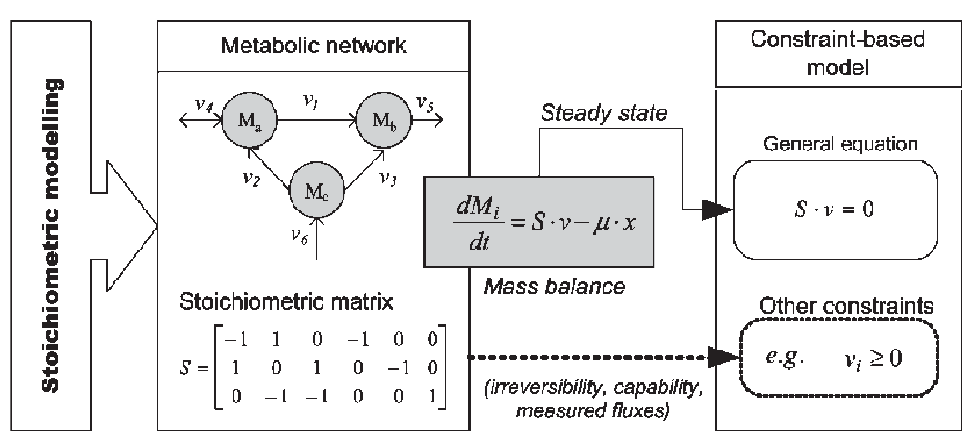
\includegraphics[width=0.8\textwidth]{Figures/fig1.png}
    \caption{Principe de la modélisation stochiométrique}
    \label{fig:stochio modelling}
\end{figure}

\end{document}
